\chapter{The Compost Bomb Instability in the Continuum Limit}
\label{chapter:continuous_compost_bomb}
\graphicspath{{continuous_compost_bomb/figs/}}

To begin the research section of this thesis, I will examine a specific example of a tipping point, namely the `Compost Bomb'. The
Compost Bomb instability refers to a proposed uncontrolled increase in soil temperature. This instability is caused when sufficiently rapid
atmospheric warming increases soil heterotrophic respiration which, in turn, heats the soil further. This generates a runaway
effect in which soil temperatures rise rapidly. I will investigate this process, neglected in Earth System Models, but which has thus far been analysed with a conceptual
model using ordinary differential equations. That model is deliberately idealised without any representation of the spatial structure of soils.
I confirm using a partial differential equation framework that this runaway effect still occurs when accounting for soil depth.
Using this newer representation I investigate the forcing parameters that make soils vulnerable to this instability. In particular, I find that the effect of
dangerously large seasonal cycle variations in air temperature can create plausible conditions for a `compost bomb' thermal instability.
\\\\
This chapter is based on a published paper, `The Compost Bomb Instability in the Continuum Limit' \parencite{Clarke2021}.

 \section{Introduction}
\label{section:compost_bomb_intro}
Coupled climate-carbon cycle Earth System Models (ESMs) show that rising temperatures will cause carbon cycle feedbacks that accelerate global
warming further \parencite{Cox2000}. Although the magnitude of the increase remains uncertain, a major contributing factor is the
response of the land carbon cycle to increased temperatures \parencite{Friedlingstein2006,Arora2020}. Over the last decade, there has therefore been a strong focus on improving
models of the expected response of terrestrial carbon to global warming.

The largest uncertainties are associated with the response of soil carbon to warming \parencite{Varney2020}.
The Jenkinson effect \parencite{Jenkinson1991} is a positive carbon cycle feedback related to the soil. Heterotrophic respiration converts
organic matter held in soils into \ce{CO2}. At higher temperatures the rate of this reaction increases, leading to
larger emissions of \ce{CO2} from soils. However, a key aspect of heterotrophic respiration, ignored by ESMs \parencite{Arora2020}, is that due to respiration being
an exothermic reaction, the released heat must raise the temperature of the soils it occurs in. This biogeochemical heating has been shown
to be important in the thawing of permafrosts \parencite{Khvorostyanov2008,Khvorostyanov2008a}.

Furthermore, because the rate of respiration increases with temperature, the biogeochemical heating will tend to
further increase the rate of respiration. This positive feedback creates the possibility of a tipping point, in which
runaway respiration also significantly increases the soil temperature.

This runaway potential was first investigated in \cite{Luke2011}. The Luke and Cox model (hereafter referred to as the LC10 model)
showed an instability if the rate of increase of air temperature was large compared to the soil turnover time. They dubbed this instability
the `compost bomb' due to the known capability of compost heaps to self-heat \parencite{Nelson2007,Sidhu2007,Browne1929}.

A range of climate tipping points have been observed in
paleoclimate records \parencite{Alley2003}, and both expert opinion \parencite{Lenton2008} and ESMs \parencite{Drijfhout2015} raise the possibility that they may be triggered this century by climate change.
These tipping points associated so far with the behaviour of the Earth system are believed to
correspond to bifurcations. The mechanisms underpinning the compost bomb instability are more unusual in that this is an example of rate-dependent tipping \parencite{Ashwin2012}.

This rate-dependence was analysed mathematically
by~\cite{Wieczorek2011} where the compost bomb was studied as an `excitable' system in which critical rates
were calculated analytically. They found that when the air temperature was
raised sufficiently slowly the system could follow the steady state equilibrium. However, when the air temperature was raised more rapidly,
the system was unable to adapt sufficiently quickly to the new equilibrium and thus tipped.

Here a focus is on the compost bomb instability in response to the seasonal cycle. In this case the timescale of the forcing (1 year) is much faster than the response timescale of the soil carbon
(decades), and the soil carbon can be treated as a prescribed time-invariant quantity (this is the `compost bomb limit' of LC10). 

Some limitations of the LC10 model are that it neglects important thermal processes and soil structure, and in particular vertical variation.
For example, as a `single box' model, it assumes that the soil is well represented by averaged quantities, such as an average soil temperature,
when in fact these quantities can be quite heterogeneous \parencite{Gedney2003}.

By definition, box models neglect processes such as heat diffusion which tend to suppress regions of unusually high temperature. Hence an initial assumption might be
that diffusive damping may make the compost bomb harder to trigger. Additionally, the LC10 model assumes a single pool of carbon, rather than a spatially extended distribution, which might
increase the possibility for a compost bomb.

Despite these caveats, the LC10 model captures the essence of the system. The aim is to add realism to the LC10 model by considering the vertical structure and heat conductivity of the soil.
The new model will consist of a one dimensional soil column in which heat can diffuse and soil carbon
decreases exponentially with depth. Whether or not an instability still exists in this model will be investigated.

The compost bomb has generally been considered in relation to an upward decadal timescale linear ramp in air temperature, which is an idealisation of the change in air temperature due to
human caused climate change. However, there is also the possibility of
rate-induced tipping by the sinusoidal variations in air temperature caused by the diurnal and seasonal cycles. These possibilities are investigated here, to see if there exist
features of these oscillations that may raise the risk of a compost bomb.


\section{LC10 Single Box Conceptual Model}
\label{sec:lc10}
The compost bomb instability is based on the idea that heterotrophic respiration in the soil is both an exothermic reaction \parencite{Thornley1971} and
also a reaction whose rate increases with temperature. Hence this reaction could lead to a scenario of thermal runaway, where respiration warms the soil which increases respiration further.
The rate of respiration is often modelled with a $Q_{10}$ form \parencite{Kirschbaum1995} for temperature dependence.
In this representation the reaction rate increases by a factor $Q_{10}$
for every \SI{10}{\degreeCelsius} of temperature increase.
Hence the specific rate of respiration, $r(T_s)$ (\si{\per\square\meter\per\second}) can be modelled as $r(T_s) = r_0 Q_{10}^{\left(T_s - T_{\mathrm{ref}}\right)/10}$
where $T_s$ (\si{\degreeCelsius}) is the soil temperature and $r_0$ is the reaction rate at
$T_{\mathrm{ref}}$. The rate of reaction also increases in proportion to the available substrate, here soil carbon $C_s$ (\si{\kilo\gram\carbon\per\square\meter}).
The $Q_{10}$ form implies an exponential dependence of the specific respiration rate on temperature:  $r(T_s)=r_0 \exp\left(\alpha\left(T_s-T_{\mathrm{ref}}\right)\right)$, where
$\alpha = \log Q_{10}/10$. The soil carbon is increased by Net Primary Production (NPP)
$\Pi$ (\si{\kilo\gram\carbon\per\square\meter\per\second}) and decreased by heterotrophic respiration. Introducing the parameters $A$ (\si{\joule\per\kilo\gram\carbon}), the specific heat
of respiration, $\mu_A$ (\si{\joule\per\square\meter\per\kelvin}) the areal soil heat capacity and $\lambda$ (\si{\watt\per\square\meter\per\kelvin})
the soil-to-atmosphere heat transfer coefficient leads to the LC10 model:
\begin{subequations}

  \label{eq:lc10}
 \begin{align}
   \mu_A\dv{T_s}{t} &= -\lambda (T_s - T_a) + AC_sr_0e^{\alpha (T_s - T_{\mathrm{ref}})}, \label{subeq:lc10_temperature}\\
  \dv{C_s}{t} &= \Pi - C_sr_0e^{\alpha (T_s - T_{\mathrm{ref}})}.  \label{subeq:lc10_soil_carbon}
 \end{align}
\end{subequations}
The model assumes that in the absence of biogeochemical heating the soil temperature equilibrates to the atmospheric temperature $T_a$. The amount of soil carbon is set by the equilibrium balance
between $\Pi$ and heterotrophic respiration.  
If the decrease in soil carbon is too slow to offset an increase in air temperature, the compost bomb instability is triggered, corresponding mathematically to an instability in which
$T_s$ is `excited' to a very large value, well in excess of \SI{100}{\degreeCelsius}. This model implies a value for the equilibrium soil carbon
\begin{equation}
  \label{eq:equilibrium_soil_carbon}
  C_s^{\mathrm{eq}} = \frac{1}{r_0}e^{-\alpha \left( T_a - T_{\mathrm{ref}}\right)} \Pi e^{-\Pi/\Pi_c}
\end{equation}
where $\Pi_c = \lambda /\alpha A$. This equilibrium value is obtained by setting the derivatives in \cref{eq:lc10} to zero.

\section{Continuum Model With Vertical Depth}
\label{sec:continuum_model}
To investigate the effects of the representation of spatial variability in the vertical $z$ (\si{\meter}) direction the soil column is
modelled as existing on a semi-infinite line, which extends from the surface at $z = 0$ down to $z = -\infty$. It is assumed that soil carbon
falls exponentially with depth, over a characteristic distance of $H$. The soil temperature is modelled by a reaction-diffusion system, in which heat is generated
by heterotrophic respiration and diffused vertically. The conductivity of the soil is given by $\kappa$ (\si{\watt\per\meter\per\kelvin}) \parencite{Best2005},
it has heat capacity $\mu_V$ (\si{\joule\per\cubic\meter\per\kelvin}) and contains a total amount $C_s$ of soil carbon. Therefore the heat equation
for the soil temperature $T_s(z,t)$ becomes:
\begin{equation}
  \label{eq:one_d_model}
  \mu_V \pdv{T_s}{t} = \kappa \pdv[2]{T_s}{z} + \frac{AC_sr_0}{H}e^{\alpha (T_s - T_{\mathrm{ref}})}e^{z/H}.
\end{equation}
At $z=-\infty$ a no flux boundary condition is imposed.
At the upper boundary the soil temperature is controlled by the turbulent heat flux from the atmosphere which has temperature
$T_{a0} + \delta T_a(t)$, where $T_{a0}$ represents a background mean temperature and $\delta T_a(t)$ a time dependent warming. Mathematically:

\begin{subequations}
  \label{eq:dimensional_bcs_nonuniform}
  \begin{align}
  \pdv{T_s}{z} &= 0 \quad \mathrm{at} \quad z = -\infty,\label{subeq:dimensional_bcs_nonuniform_lower} \\[1ex] 
  - \kappa\pdv{T_s}{z} &=   \lambda\left(T_s\left(0,t\right) - T_{a0} - \delta T_a\left(t\right)\right) \quad \mathrm{at}\quad z = 0.\label{subeq:dimensional_bcs_nonuniform_upper}
  \end{align}
\end{subequations}

Here the parameter $\lambda$ characterises the turbulent heat transfer from the atmosphere to the top layer of the soil.
$C_s$ is set to the equilibrium value using \cref{eq:equilibrium_soil_carbon} where the air temperature is taken to be $T_{a0}$. This approximation
is justified provided the system is investigated on timescales short relative to the turnover time of soil carbon, which is on the order of many decades \parencite{Varney2020}. 

Throughout this study I undertake the mathematical investigation using nondimensional values. However, to aid understanding I plot certain figures
using dimensional units, with standard values given in \cref{tab:standard_values}. It should be noted however that these parameters are choices I have made,
and different choices will lead to different figures, whereas the nondimensional plots are valid for all parameter choices.

\begin{table}
  \centering
  \begin{tabular}{@{}llll@{}}
  Parameter    & Symbol & Equation & Value                                          \\ \midrule
  Net Primary Productivity &$\Pi$     &\ref{subeq:lc10_soil_carbon} &\SI{0.5}{\kilo\gram\carbon\per\year}           \\
  Temperature response of respiration &$Q_{10}$   &\ref{eq:one_d_model} & 2.5  \\
  Characteristic Soil Depth &$H$       &\ref{eq:one_d_model} &\SI{0.4}{\meter}                               \\ 
  Soil Thermal Conductivity &$\kappa$  &\ref{eq:one_d_model} &\SI{0.16}{\watt\per\meter\per\kelvin}          \\
  Specific Heat of Respiration &$A$       &\ref{eq:one_d_model} &\SI{3.9e9}{\joule\kilo\gram\per\carbon}        \\
  Volumetric Heat Capacity&$\mu_V$   &\ref{eq:one_d_model} &\SI{1.0}{\mega\joule\per\cubic\meter\per\kelvin} \\
  Heat Transfer Coefficient &$\lambda$ &\ref{subeq:dimensional_bcs_nonuniform_upper} &\SI{10}{\watt\per\square\meter\per\kelvin} \\
  Average Air temperature   &$T_{a0}$  &\ref{subeq:dimensional_bcs_nonuniform_upper} &\SI{0.0}{\degreeCelsius}
\end{tabular}
\caption{Parameter values used to produce the figures in this study.}
\label{tab:standard_values}
\end{table}
\subsection{Numerical Investigation}
\label{sec:numerical_investigation}
The continuum model was integrated in both space and time, and it was found that it can give rise to a compost bomb instability.
The PDE, \cref{eq:one_d_model}, was solved using the `method of lines' technique \parencite{Schiesser2012}. It was discretized spatially into 100 equally spaced intervals.
The spatial derivatives were approximated using central differences. This was then integrated using
the backwards differentiation formula \textsc{bdf} method from the scipy library \parencite{Virtanen2020}. The \textsc{bdf} method was chosen as it is well suited to stiff problems.
If scipy's solver could not find a solution, then it was assumed that compost bomb had occurred.

This is a first piece of evidence that the results of the LC10 model remain when soil depth is taken into account. \Cref{fig:vertical_profiles}
is a plot of the temperature profile of soil at different times, initialised to be in equilibrium, undergoing the compost bomb thermal runaway after five months.
$\delta T_a$ was set to a  a sinusoid of frequency one year. \Cref{fig:vertical_profiles} shows that
the instability remains in the continuous case, and it is not prevented by diffusion.

\begin{figure}
  \centering
  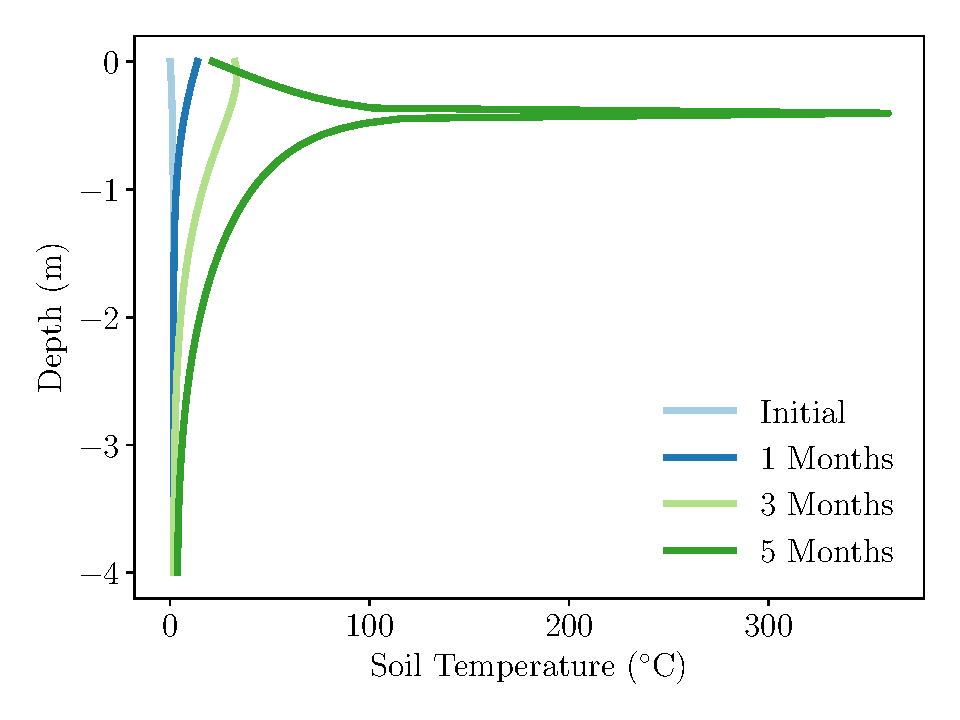
\includegraphics[scale=0.5,keepaspectratio]{seasonal_cycle_profiles}
  \caption[Vertical profile of soil temperature]{Vertical temperature profiles of soil undergoing a compost bomb thermal runaway when subject to a seasonal cycle of temperatures with amplitude \SI{32.5}{\degreeCelsius}.}
  \label{fig:vertical_profiles}
\end{figure}
\subsection{Consistency of the continuum model with LC10}
\label{sec:consistency_with_LC10}
In this subsection the LC10 model and continuum model are compared numerically. The level of soil carbon is chosen such that the soil temperature is
initially in an equilibrium state with $\delta T_{a} = 0$. The models are then integrate forward in time with $\delta T_a$ constant and greater than zero.
For sufficiently large values of $\delta T_a$ the system has an instability. The smallest value of $\delta T_a$ for which this is true is referred to
as the `critical warming level', because if air temperatures were increased by this amount quickly with respect to the soil carbon turn over time,
an instability would be triggered.

This critical warming is plotted, as a function of $\kappa$ in \cref{fig:comparison_with_lc10}.
Also overlaid is the warming required to cause a compost bomb in the LC10
model. Also shown is the amplitude of the seasonal cycle needed to cause a compost bomb.
It can be observed that as $\kappa\rightarrow\infty$ the vertical structure matters less and the continuum result asymptotes to the LC10 case. In addition, the soil is more stable
to seasonal cycle oscillations than instantaneous jumps. This `overshoot' behaviour \parencite{Ritchie2019,Ritchie2021} is due to the fact that soil temperatures do not instantly respond to the seasonal cycle.
Surprisingly for smaller values of $\kappa$ the critical warming is actually lower in the continuum case than the LC10 case,
despite the damping effects of diffusion.
\begin{figure}
  \centering
  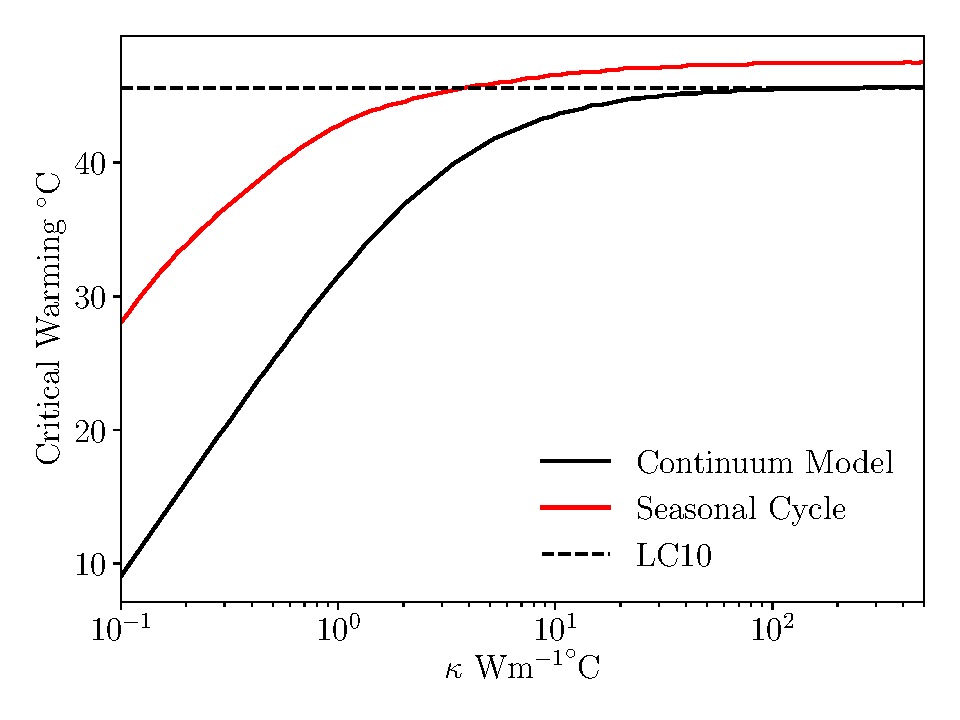
\includegraphics[keepaspectratio,scale=0.5]{dimensional_continuum_vs_lc10}
  \caption[Critical warming level in the continuum compost bomb]{The warming required to make the continuum model unstable as a function of $\kappa$, compared to the LC10 model.
    Also plotted on is the seasonal cycle amplitude required for this instability.}
  \label{fig:comparison_with_lc10}
\end{figure}

To investigate this further, the LC10 model will be derived from the continuum case. This is done by vertically averaging \cref{eq:one_d_model}.
Vertically averaged quantities are denoted by
$\left\langle q \right\rangle = \frac{1}{H}\int_{-\infty}^0 q \mathrm{d}z$.  Begin by integrating \cref{eq:one_d_model} over the vertical domain:
\begin{equation}
  \label{eq:vertical_integration}
  \mu_V \dv{t} \int_{-\infty}^0 T_s \, \mathrm{d} z =
  \kappa \eval{\pdv{T_s}{z}}_{z=0}
  - \kappa \eval{\pdv{T_s}{z}}_{z=-\infty} +
  \frac{AC_sr_0}{H} \int_{-\infty}^0 e^{\alpha \left(T_s - T_{\mathrm{ref}}\right)} e^{z/H} \, \mathrm{d} z.
\end{equation}
Applying boundary conditions (\cref{eq:dimensional_bcs_nonuniform}) gives
\begin{equation}
  \label{eq:vertical_integration_after_bc}
  \mu_V H \dv{\left\langle T_s \right\rangle}{t} = -\lambda \left( T_s\left(0,t\right) - T_{a0}
    - \delta T_a\left(t\right)\right) + \frac{AC_sr_0}{H}\int_{-\infty}^0 e^{\alpha \left(T_s - T_{\mathrm{ref}}\right)} e^{z/H} \, \mathrm{d} z.
\end{equation}

Assuming the vertical distribution of soil carbon does not affect the average value too much and setting $\mu_A = \mu_VH$ gives 
\begin{equation}
  \label{eq:vertically_averaged}
  \mu_A \dv{\left\langle T_s \right\rangle}{t} = -\lambda \left( T_s\left(0,t\right) - T_{a0} - \delta T_a\left(t\right)\right) +
  AC_sr_0\left\langle e^{\alpha \left(T_s - T_{\mathrm{ref}}\right)}\right\rangle.
\end{equation}
This is equivalent to the LC10 model if $T_s(0,t) \approx \left\langle T_s \right\rangle$ and $\left\langle e^{\alpha T_s}\right\rangle \approx e^{\alpha \left\langle T_s \right\rangle}$.
These approximations become exact when $T_s$ is not a function of $z$, which occurs when $\kappa \rightarrow \infty$, as shown in \cref{fig:comparison_with_lc10}.
Note however that because $\left\langle e^{\alpha T_s} \right\rangle \ge e^{\left\langle \alpha T_s \right\rangle}$ the LC10 model underpredicts the amount of respiration
in soils when $\kappa$ is finite, and so the LC10 model will need a higher amount of warming to trigger a compost bomb.

  
\subsection{Existence of the Compost Bomb in the Continuum Case}
\label{sec:existence_of_compost_bomb}
Now that there is numerical evidence for a compost bomb in the continuum case, this will be investigated analytically. In the approximation where soil carbon is constant,
the rate dependent tipping feature of the model is lost, and instead it reverts to a classical bifurcation-induced tipping problem.
Consider the case where $\delta T_a$ is a constant, given by the temperature increase relative to the long term background state, $T_{a0}$, which is refereed to as an atmospheric warming.
In this case $\delta T_a$ is the bifurcation control parameter.
To begin the following nondimensionalisations are made:
\begin{subequations}
  \label{eq:nondimensionalisations}
  \begin{align}
    \theta &= \alpha\left(T_s - T_{a0}\right) \label{subeq:nondimensionalisations_soil_temperature}\\
    \delta\theta_a &= \alpha \delta T_a \label{subeq:nondimensionalisations_air_temperature}\\
    x &= \frac{\lambda z}{\kappa}  \label{subeq:nondimensionalisations_depth}\\
    \tau &= \frac{\lambda^2 t}{\kappa\mu_V} \label{subeq:nondimensionalisations_time}\\
    \widetilde{\Pi} &= \Pi/\Pi_c \label{subeq:nondimensionalisations_npp}
  \end{align}
\end{subequations}
then \cref{eq:one_d_model,eq:dimensional_bcs_nonuniform} become
\begin{subequations}
  \label{eq:nondimensional_model_nonuniform}
  \begin{align}
  \pdv{\theta}{\tau} &= \pdv[2]{\theta}{x} + \mathcal{W} e^{\theta}e^{x/D} \label{subeq:nondimensional_model_nonuniform_reaction_diffusion}\\
  \pdv{\theta}{x} &= 0\quad \mathrm{when} \quad x=-\infty \label{subeq:nondimensional_model_nonuniform_bcs_upper}\\
  -\pdv{\theta}{x} &= \theta(0,t) - \delta\theta_a(t) \quad \mathrm{when} \quad x=0             \label{subeq:nondimensional_model_nonuniform_bcs_lower}
  \end{align}
\end{subequations}
The nondimensionalisation process reveals two parameter clusters $D = H\lambda/\kappa$ and $\mathcal{W} = \widetilde{\Pi}e^{-\widetilde{\Pi}}/D$, which
correspond to a nondimensional soil thermal depth and a nondimensional respiration strength. Note that $\theta$ and $\delta\theta_a$ should be interpreted as (nondimensional) temperatures
relative to the background air temperature, so in particular $\delta\theta_a$ is a temperature anomaly.

It will now be shown that the model defined by \cref{eq:nondimensional_model_nonuniform} only has an equilibrium state for low levels of atmospheric warming, $\delta\theta_a$.
First a change of variables is made to reveal the first integral of the steady-state of 
\cref{subeq:nondimensional_model_nonuniform_reaction_diffusion}. Then a second integration followed by a change of variables reveals a standard integral with a
well-known solution.

Let $\delta\theta_a$ be constant, set $\partial_{\tau}\theta = 0$, and then let $\psi = \theta + x/D$. Then \cref{subeq:nondimensional_model_nonuniform_reaction_diffusion} becomes
\begin{equation}
  \dv[2]{\psi}{x} + \mathcal{W}e^{\psi} = 0.
\end{equation}
Multiplying this by $\dv*{\psi}{x}$ and integrating gives
\begin{equation}
  \int\dv{\psi}{x}\dv[2]{\psi}{x}\,\mathrm{d}z + \int\mathcal{W}\dv{\psi}{x}e^\psi\,\mathrm{d}{x} = 0
\end{equation}
\begin{equation}
  \int \dv{x}\left(\frac{1}{2}\left(\dv{\psi}{x}\right)^2\right)\,\mathrm{d}x + \mathcal{W} \int \dv{e^{\psi}}{x} \, \mathrm{d}x = 0
\end{equation}
\begin{equation}
  \frac{1}{2} \left(\dv{\psi}{x}\right)^2 + \mathcal{W}e^{\psi} = \frac{1}{2} c_1
\end{equation}
with $c_1$ a constant.
Rearranging and recognising that this is a separable differential equation gives
\begin{equation}
  \int \frac{\mathrm{d}\psi}{\sqrt{1 - 2\mathcal{W}c_1^{-1} e^{\psi}}} = \pm\sqrt{c_1} \int \mathrm{d}x = c_2 \pm \sqrt{c_1} x 
\end{equation}
where $c_2$ is another integration constant. The right hand side is then reduced to a standard integral \parencite{riley2006}
with the substitution $u = \left(1 - \frac{2\mathcal{W}}{c_1} e^{\psi}\right)^{1/2}$, giving
\begin{equation}
  \int \frac{\mathrm{d}\psi}{\sqrt{1 - 2\mathcal{W}c_1^{-1} e^{\psi}}} = \int \frac{2}{u^2 - 1} \,\mathrm{d}u = \artanh u. 
\end{equation}
Inverting this then leads to
\begin{equation}
  \sqrt{1 - 2\mathcal{W}c_1^{-1} e^{\psi}} = \tanh\left(c_2 \pm \sqrt{c_1} x\right)
\end{equation}
and thus
\begin{equation}
  \psi = \log \frac{c_1}{2\mathcal{W}} + \log \left(1 - \tanh^2 \left(c_2 \pm \sqrt{c_1} x\right)\right).
\end{equation}
Using the Pythagorean identity \parencite{riley2006} this can be reduced to
\begin{equation}
  \psi = \log \frac{c_1}{2\mathcal{W}} + 2\log \left(\sech \left(c_2 \pm \sqrt{c_1} x\right)\right).
\end{equation}
In terms of $\theta$, the solution is
\begin{equation}
  \label{eq:nondimensional_model_nonuniform_solution_general}
  \theta = \log \frac{c_1}{2\mathcal{W}} + 2 \log \sech \left( \frac{c_2 \pm \sqrt{c_1} x}{2}\right) - \frac{x}{D}
\end{equation}
Applying the boundary condition at $x = -\infty$ implies that $c_1 = \frac{1}{D^2}$.  The solution becomes:
\begin{equation}
  \label{eq:nondimensional_model_nonuniform_solution_one_bc}
  \theta = \log \frac{1}{2\mathcal{W}D^2} + 2 \log \sech \left( \frac{1}{2} \left(c_2 \pm \frac{x}{D}\right)\right) - \frac{x}{D}
\end{equation}
Now applying the boundary condition at $x = 0$ gives
\begin{equation}
  \label{eq:nondimensional_model_nonuniform_upper_boundary_condition}
  \pm\frac{1}{D}\tanh \frac{c_2}{2} - 2 \log \sech \frac{c_2}{2} = -\frac{1}{D} - \log 2\mathcal{W}D^2 - \delta\theta_a.
\end{equation}
Denoting the left-hand side of this equation as $F(c_2)$, it can be shown that $F$ has a minimum. To see this note that $F$ is a continuous function which
for $|c_2| \rightarrow \infty$ behaves like $F(c_2) \sim 2|c_2|$ so it follows %from Rolle's Theorem\parencite{Bourbaki2004}
that $F$ has a minimum. Hence for sufficiently large $\delta\theta_a$, the right-hand side will always
be less than the left-hand side. This means there is no equilibrium solution, consistent with a compost bomb having been triggered.

To determine the critical level of $\delta\theta_a$ to cause a compost bomb,
the $c_2$ that satisfies $F'(c_2) = 0$ must be found and substituted back into \cref{eq:nondimensional_model_nonuniform_upper_boundary_condition}. The derivative of $F$
is
\begin{equation}
  F'(c_2) = \pm \frac{1}{2D}\sech^2 \frac{c_2}{2} + \tanh \frac{c_2}{2} = \pm \frac{1}{2D}\left(1 - \tanh^2 \frac{c_2}{2}\right) + \tanh \frac{c_2}{2} 
\end{equation}
so that $F'(c_2) = 0$ can be solved for $\tanh c_2$ and so \cref{eq:nondimensional_model_nonuniform_upper_boundary_condition} becomes
\begin{equation}
  \label{eq:nondimensional_model_nonuniform_critical_warming}
  \delta\theta_a^{\mathrm{crit}} = \log \left(2D\sqrt{D^2 +1} - 2D^2\right) -1 + \frac{1}{D} \sqrt{D^2 + 1} - \frac{1}{D} - \log 2\mathcal{W}D^2
\end{equation}
Note that for sufficiently large values of $\mathcal{W}$, the right-hand side of this equation is negative, which can be interpreted as the soil being inherently unstable without any warming.

As $\mathcal{W}$ is a function of $\widetilde{\Pi}$ and $D$, specifying $\widetilde{\Pi}$ and $D$ is enough to determine $\delta\theta_a^{\mathrm{crit}}$, through
\cref{eq:nondimensional_model_nonuniform_critical_warming}. The critical maximum warming is plotted in \cref{fig:critical_theta_a} for a range of $\widetilde{\Pi}$ and $D$ values.
\Cref{fig:critical_theta_a} shows the critical warming, above which no equilibrium solutions exist, corresponding to triggering a compost bomb.
Increasing the `fuel', $\widetilde{\Pi}$, decreases the warming
required to trigger a compost bomb. Furthermore, the figure shows that in this model, soils with larger $D$, corresponding to soils that are well insulated and have a
soil carbon with a weak dependence on depth, are more unstable.
\begin{figure}
  \centering
  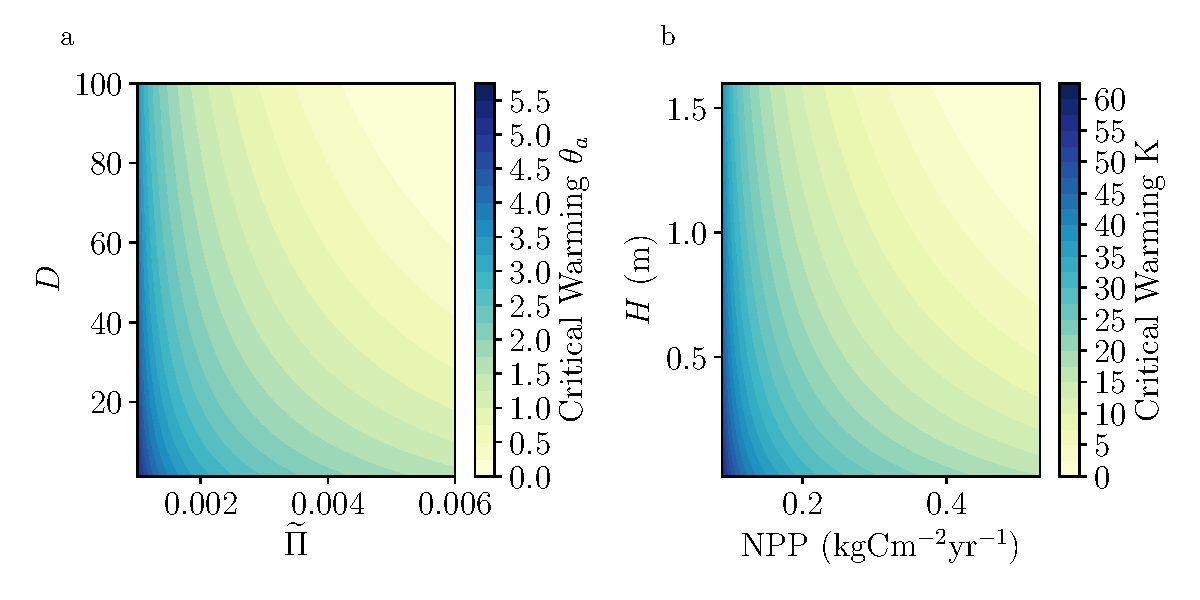
\includegraphics[keepaspectratio,scale=0.5]{static_dim_and_nondim}
  \caption[Critical warming to trigger a compost bomb]{\textbf{Panel a}: the relationship between nondimensional soil carbon $e$-folding depth $D$,
    nondimensional NPP $\widetilde{\Pi}$ and the critical warming required to cause a compost
    bomb $\delta\theta_a$. \textbf{Panel b}: Also plotted is a dimensional version using the standard parameters in \cref{tab:standard_values}}
  \label{fig:critical_theta_a}
\end{figure}


\section{Vulnerability To Seasonal Cycle}
\label{sec:seasonal_cycle}
The compost bomb instability is a rate-induced instability. To trigger the compost bomb instability, the rate of increase in air temperature needs to be fast
relative to the rate of decrease of soil carbon. Prior work \parencite{Luke2011} examined a linear increase in air temperature, corresponding to the increase in
mean air temperature being caused by anthropogenic influence.

However, air temperature varies on multiple timescales. Two important modes of rapid air temperature change (relative to the timescale of soil
carbon) are the diurnal and seasonal cycles. Suppose $\delta T_a$ varies sinusoidally,
\begin{equation}
  \label{eq:sinusoidal_forcing}
  \delta T_a(t) = \Delta T_a \sin \frac{2\pi t}{T}
\end{equation}
and numerically integrate \cref{subeq:nondimensional_model_nonuniform_reaction_diffusion} for a range of
forcing periods, using the standard parameters in \cref{tab:standard_values}. Sufficiently large forcing amplitudes will lead to a compost bomb.
These are plotted in \cref{fig:forcing_frequency_vs_amplitude}.
\begin{figure}
  \centering
  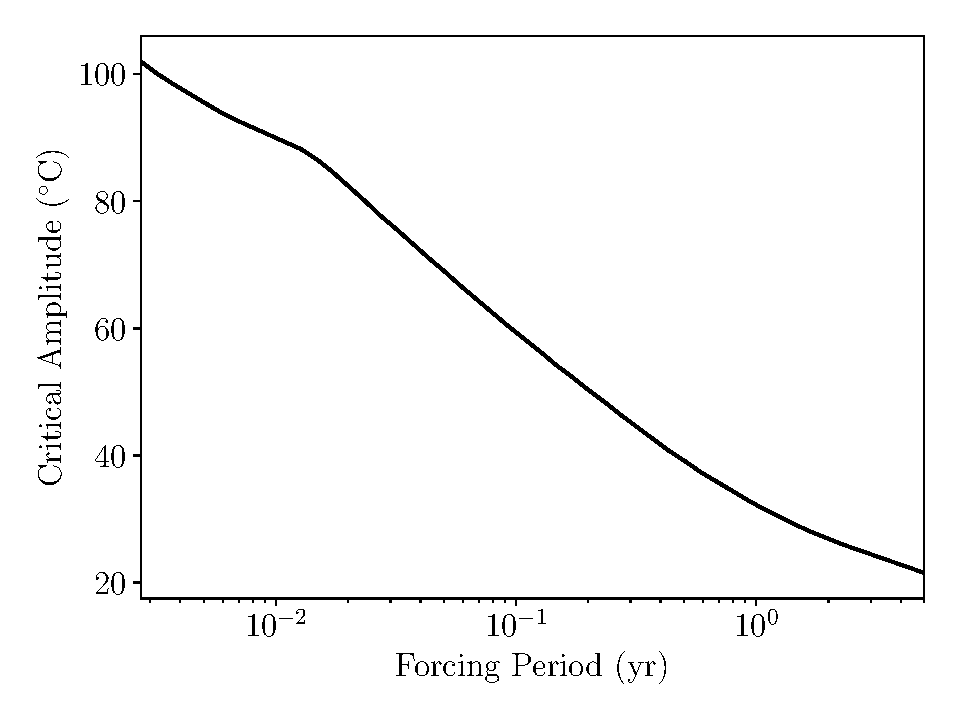
\includegraphics[scale=0.5,keepaspectratio]{critical_amplitude_vs_period}
  \caption[Critical warming for periodic forcing]{The relationship between forcing period $T$ and the amplitude of the minimum near surface air temperature changes required to trigger a compost bomb.}
  \label{fig:forcing_frequency_vs_amplitude}
\end{figure}

Whilst the rate dependence alone would suggest that higher frequency oscillations are more unstable,
high frequency oscillations can be too rapid to affect the soil temperature. Such high frequencies are in effect `averaged out', as the air cannot heat the soil rapidly enough to
have an effect deeper in the soil. Hence diurnally driven compost bombs are unlikely except at very high and unrealistic amplitudes.

In particular from \cref{fig:forcing_frequency_vs_amplitude}, 
the amplitudes required to cause a compost bomb from the very high frequency diurnal cycle are about \SI{100}{\degreeCelsius}, which is implausibly large.
However for oscillations corresponding to timescales of the annual seasonal cycle, the magnitude is around \SI{30}{\degreeCelsius}. This remains large,
but such variations occur in high latitude, soil carbon rich ecosystems, for instance in parts of Siberia \parencite{Peixoto1992}.

The possibility of a seasonal cycle triggered compost bomb was investigated and plotted in \cref{fig:critical_amplitude_to_be_triggered_by_the_seasonal_cycle},
by scanning across the two nondimensional parameters.
This shows that for a variety of plausible parameters, a large seasonal cycle could trigger a compost bomb. Soils with larger $\widetilde{\Pi}$ are more susceptible to a seasonal
cycle driven compost bomb as they have more `fuel'. However, in marked contrast to the conditions for the existence of an equilibrium, shallower soils are more susceptible to seasonal cycle driven
compost bombs. This susceptibility can be understood as the atmosphere being able to warm larger fractions of shallower soils per unit of time.


\begin{figure}
  \centering
  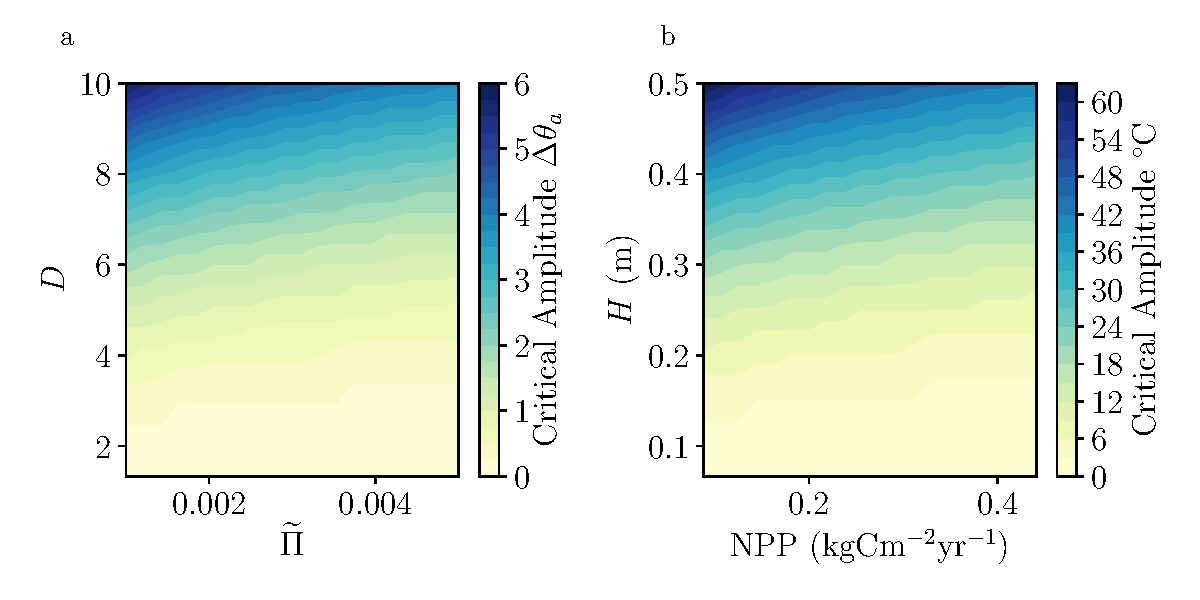
\includegraphics[scale=0.5,keepaspectratio]{seasonal_dim_and_nondim}
  \caption[Critical seasonal cycle for a compost bomb]{\textbf{Panel a}: the relationship between nondimensional respiration, soil depth and the seasonal cycle amplitude required to cause a compost bombs.
    For typical values of $Q_{10}$, the seasonal cycle could trigger a compost bomb. \textbf{Panel b}: Also plotted is the dimensional version, where the standard value
    of $\kappa$ is modified to \SI{0.5}{\watt\per\meter\per\kelvin} so make the $H$ values more realistic.}
  \label{fig:critical_amplitude_to_be_triggered_by_the_seasonal_cycle}
\end{figure}

\section{Discussion}

The purpose of this research is to determine features of raised near-surface temperature that could trigger thermal runaway in soils, a process called a `compost bomb'.
The compost bomb instability was originally identified in a single box model. The overarching finding of this chapter is that when accounting for vertical heterogeneity,
thermal runaway still occurs. For all finite values of thermal conductivity, I find these temperature thresholds are lower than those in the LC10 model, which I attribute
to the strongly nonlinear respiration response to temperature.

The analysis undertaken suggests there are two important nondimensional parameters, $D$ and $\mathcal{W}$ which characterise the `thermal thickness' and energy output
of respiration respectively.
%Nondimensionalisation supports this balance of two dominant factors,
%by collapsing the governing equations to parameters $D$ and $\mathcal{W}$, that characterise the physical thermal aspects and respiration strength respectively.
%For our standard set of parameters, a rapid increase followed by a sustained temperature of order \SI{10}{\degreeCelsius} may push the soil system into the unstable regime.
%Besides discovering dangerous jumps in critical near-surface air temperature, above which there is no stable state, I also investigate the vulnerability to seasonal cycles in air temperature.
%I find that it is plausible that annual cycles of around \SI{30}{\degreeCelsius} risk uncontrolled warming in soils.
However, I have created a deliberately simplified model of the compost bomb. This has the advantage of being analytically tractable, yet ignores certain processes. Most obviously,
I assume soil carbon is in equilibrium. This is not an unreasonable assumption however as I consider short enough timescales where this is approximately true.
More importantly I neglect the role of soil moisture. Although this is not a thorough analysis, I offer some justification for why this model captures
the essential features of the system. The addition of soil moisture has two principal effects.

Firstly, it affects the amount of respiration in the soils. In the framework of our model, weakening respiration corresponds to decreasing $\mathcal{W}$,
a nondimensional parameter that encodes the amount of soil carbon, the heat released from respiration and the thermal properties of the soil. 
Although this affects the precise value for the air temperature warming that leads to a compost bomb, for any $\mathcal{W} > 0$ there is still a critical level of warming that produces a compost bomb.

Secondly soil moisture affects heat transport by setting the conductivity of the soil. However the thermal conductivity can be
modelled as varying linearly with soil moisture \parencite{Best2011}, whereas respiration has an exponential dependence on temperature. Therefore, temperature variations
should play a more important role than moisture variations in the dynamics of the compost bomb.
%It is reasonable to neglect seasonal changes in the conductivity
%when compared to seasonal changes in respiration, as respiration varies exponentially with temperature.

%However, even with these approximations, I have added to the evidence base of the plausibility of self-igniting fires in soils, and with an equation set that accounts explicitly for depth variation.
%Whilst adding a feature that can cause `blow-up' requires great care, I would encourage ESM developers to examine this effect in more complicated models to discover the situations in which it is important.

\section{Conclusion}
\label{sec:conclusion}
In this chapter I present an advance in the realism of compost bomb models, by accounting for the vertical structure of the soils. I have found that even accounting
for the diffusive effects of vertical structure, compost bombs can still occur. Furthermore, for realistic levels of heat diffusion,
warming levels required to initiate the instability are much smaller than in the LC10 case. For the set of parameters investigated a rapid warming of the order of \SI{10}{\degreeCelsius} is
enough to push soils into an unstable regime. Furthermore, I have also found that for annual temperature cycles of around \SI{30}{\degreeCelsius} risk triggering compost bombs.

This research adds to the evidence base that fires may self-ignite in high-latitude soils, which would have implications for the carbon cycle in these regions.
This should encourage the development of biogeochemical heating in state-of-the-art land surface models to study the situations in which biogeochemical heating is important.

